\begin{frame}
    \frametitle{\problemtitle}

    \begin{columns}
        \begin{column}[T]{.70\textwidth}
            \begin{itemize}
                \item You have $1 \leq n \leq 4 \cdot 10^5$ CPU cores and an array of $n + 1$ integers ($0 \leq a_i \leq 10^9$).
                \item Sort them by alternating between two types of rounds:
                \begin{itemize}
                    \setlength{\itemindent}{-0.5em}
                    \item First core compares $a_0$ and $a_1$, third core compares $a_2$ and $a_3$, \dots
                    \item Second core compares $a_1$ and $a_2$, fourth core compares $a_3$ and $a_4$, \dots
                \end{itemize}
                \item Determine the number of rounds that the parallel sorting algorithm runs before the array becomes sorted.
            \end{itemize}
        \end{column}

        \illustration{0.25}{cpus}{CPUs. CC0 by Martijn Boer on \href{https://flic.kr/p/2jizNX8}{Flickr}}%
    \end{columns}

    \vspace{0.5em}

    \centering
    \small
    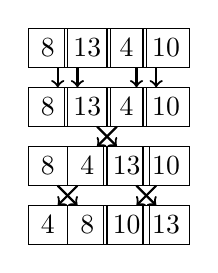
\begin{tikzpicture}[scale=0.25]
        \node[draw,rectangle,minimum size=0.5cm] at (0,9) {$8$};
        \node[draw,rectangle,minimum size=0.5cm] at (2,9) {$13$};
        \node[draw,rectangle,minimum size=0.5cm] at (4,9) {$4$};
        \node[draw,rectangle,minimum size=0.5cm] at (6,9) {$10$};

        \node[draw,rectangle,minimum size=0.5cm] at (0,6) {$8$};
        \node[draw,rectangle,minimum size=0.5cm] at (2,6) {$13$};
        \node[draw,rectangle,minimum size=0.5cm] at (4,6) {$4$};
        \node[draw,rectangle,minimum size=0.5cm] at (6,6) {$10$};

        \node[draw,rectangle,minimum size=0.5cm] at (0,3) {$8$};
        \node[draw,rectangle,minimum size=0.5cm] at (2,3) {$4$};
        \node[draw,rectangle,minimum size=0.5cm] at (4,3) {$13$};
        \node[draw,rectangle,minimum size=0.5cm] at (6,3) {$10$};

        \node[draw,rectangle,minimum size=0.5cm] at (0,0) {$4$};
        \node[draw,rectangle,minimum size=0.5cm] at (2,0) {$8$};
        \node[draw,rectangle,minimum size=0.5cm] at (4,0) {$10$};
        \node[draw,rectangle,minimum size=0.5cm] at (6,0) {$13$};

        \draw[->,thick] (0.5,8) -> (0.5,7);
        \draw[->,thick] (1.5,8) -> (1.5,7);
        \draw[->,thick] (4.5,8) -> (4.5,7);
        \draw[->,thick] (5.5,8) -> (5.5,7);

        \draw[->,thick] (2.5,5) -> (3.5,4);
        \draw[->,thick] (3.5,5) -> (2.5,4);

        \draw[->,thick] (0.5,2) -> (1.5,1);
        \draw[->,thick] (1.5,2) -> (0.5,1);
        \draw[->,thick] (4.5,2) -> (5.5,1);
        \draw[->,thick] (5.5,2) -> (4.5,1);
    \end{tikzpicture}

    Illustration of Sample Input 1, where the array is sorted after three rounds.
\end{frame}
